\documentclass[10pt,a4paper]{article}
\usepackage[utf8]{inputenc}
\usepackage[T1]{fontenc}
\usepackage{lmodern}
\usepackage[a4paper,margin=20mm]{geometry}
\usepackage{amsmath,amssymb,amsthm,bm,booktabs,array,microtype,graphicx,xcolor,hyperref}
\hypersetup{colorlinks=true,urlcolor=blue,linkcolor=blue}
\newcommand{\vf}{\rho_{\!f}}
\newcommand{\rc}{r_c}
\newcommand{\om}{\boldsymbol{\omega}}
\newcommand{\vfield}{\mathbf v}
\newcommand{\status}[1]{\textsf{#1}}
\setlength{\parskip}{0.4em}
\setlength{\parindent}{0pt}
\title{\textbf{Mathematical Evidence Registry v0.1.1}\\
\large Kelvin spectra, conditional gap thermodynamics,\\ and conservative versus effective two-sector dynamics}
\author{Independent mathematical audit of historical SST manuscripts\\\small Prepared 21 October 2026}
\date{DEVELOPMENT --- NOT PHYSICALLY CERTIFIED}
\begin{document}
\maketitle
\begin{abstract}
This release adds 22 source-traceable findings to SST Mathematical Evidence Registry v0.1.0 without changing its 379 unreviewed raw formula extractions, 41 previously curated claims, or source fingerprints. It independently examines two Kelvin-gap manuscripts and a proposed hydrodynamic dual-vacuum model. Mathematical validity, independently measured vortex dynamics, quantum interpretation, and empirical evidence are strictly separated. A Python standard-library validation suite exercises 55 regression tests (23 retained and 32 new), including dispersive scaling, Bose oscillator thermodynamics, analytic rate models and a positive-energy conservative coupled oscillator. All physical identifications remain unresolved.
\end{abstract}
\tableofcontents
\section{Source provenance and epistemic constraints}
The primary manuscripts are (i) \emph{Kelvin Mode Suppression in Atomic Orbitals: A Vortex-Filament Gap}, 10 pages; (ii) \emph{Suppression of Kelvin-Mode Thermodynamics in Atomic Orbitals}, 8 pages (historical preprint dated 14 December 2025); and (iii) \emph{Hydrodynamic Dual-Vacuum Unification}, 5 pages (1 December 2025). The first two share essentially the same proposed mechanism and are not independent evidence. Full source byte hashes appear in \texttt{results/source\_manifest.json}. All cited page numbers are physical PDF pages, not automatically assigned equation IDs.

\textbf{Provenance policy.} An equation that is mathematically correct given explicit assumptions may be retained, without validating the assumption or its proposed interpretation. A result calculated from a supplied circulation, a supplied frequency, or a chosen gap is not an independent prediction of that input. Historical summaries and prior AI assessments are discovery indexes, never primary proofs.

\section{Kelvin-wave dispersion and circulation incompatibility}
\subsection{Asymptotic dispersion: mathematically useful}
For small bending disturbances of a locally straight slender vortex filament, a commonly used long-wave relation is \cite{Saffman1992,Fetter2009}
\begin{equation}
\omega_{\rm loc}(k)=\frac{\Gamma k^2}{4\pi}\left[\ln\!\frac{1}{|k|\xi}+C_0\right],\quad |k|\xi\ll1,
\label{eq:kelvin}
\end{equation}
where circulation $[\Gamma]={\rm m^2\,s^{-1}}$, wavenumber $[k]={\rm m^{-1}}$, core length $[\xi]={\rm m}$ and the dimensionless constant $C_0$ depends on the core prescription. Hence $[\omega]={\rm s^{-1}}$. The periodic surrogate $k_m=2\pi m/L$ gives a diagnostic scale, not the actual eigenvalues of a curved or knotted loop. In particular, the removal of global translation/rotation and circulation-preserving constraints is necessary before interpreting low-$m$ branches as intrinsic modes.

The first Kelvin manuscript uses $\Gamma_{\rm paper}=h/m_e$, whereas the current SST canon defines $\Gamma_{\rm canon}=2\pi\rc v_{\rm swirl}$. These are incompatible numerical prescriptions unless a distinct circulation sector is explicitly established:
\begin{align}
\Gamma_{\rm paper}&=7.27389509\times10^{-4}\ {\rm m^2s^{-1}},\\
\Gamma_{\rm canon}&=9.68361920\times10^{-9}\ {\rm m^2s^{-1}},\\
\frac{\Gamma_{\rm paper}}{\Gamma_{\rm canon}}&=75\,115.4598.
\end{align}
Using the same geometry in Eq.~\eqref{eq:kelvin}, all frequencies scale directly with the chosen $\Gamma$. This is a change of input, not a new physical effect. The printed frequency $\omega_1=2.8\times10^{17}\,{\rm s^{-1}}$ corresponds to $\hbar\omega_1=184.299\,{\rm eV}$, not $29.5\,{\rm eV}$; both figures appear in the original manuscript's appendix (p. 8).

\begin{figure}[ht]
\centering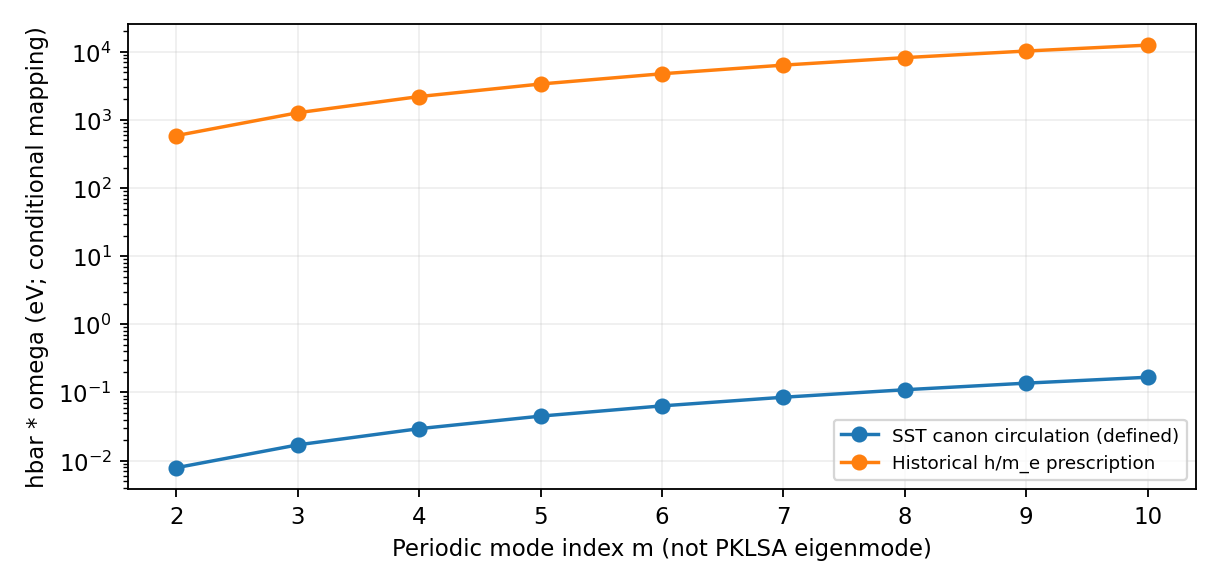
\includegraphics[width=.88\linewidth]{figures/kelvin_contract_comparison.png}
\caption{Illustrative straight-filament/periodic-wave surrogate at fixed $L=2\pi a_0$, $\xi=r_c$, $C_0=1$; $m\ge2$. \textbf{Not} the spectral output of Euler/PKLSA, and $\hbar\omega$ is an imported energy mapping.}
\end{figure}

\subsection{Finite-length spacing is not an independently derived topological gap}
A bounded periodic arclength may produce a discrete sequence of $k_m$. It does not by itself prove a universal positive \emph{topological} excitation gap; symmetry-related zero modes and curvature effects need separate treatment. The correct native test computes the linearized operator around an actual stationary/relative-periodic vortex, removes symmetry-neutral directions, and checks its eigenvalues under spatial and time refinement. A positive minimal frequency of a classical linearized system also does not independently establish a quantum excitation energy $\hbar\omega$.

\subsection{Dimensional failures in the proposed gap estimate}
The first manuscript's $\Delta_K\sim\Gamma^2/(4\pi\xi L)$ has dimensions
\[
\left[\Gamma^2/(\xi L)\right]={\rm m^2s^{-2}},
\]
a \emph{specific} energy scale, not joules. The putative tension $\vf\Gamma^2/(4\pi\xi^2)$ has units ${\rm N\,m^{-2}}$ (pressure), not ${\rm N}$ (energy per unit filament length). The actual line energy of a slender vortex typically involves $\vf\Gamma^2$ multiplied by a dimensionless logarithmic factor. A mode-specific effective inertia and finite-core dynamical model are required before any absolute gap estimate.

\section{What the Kelvin-gap thermal mathematics establishes}
\subsection{Single-mode partition function}
Assume an \emph{independent quantized bosonic harmonic mode} with excitation energy $\Delta>0$ and inverse temperature $\beta=(k_B T)^{-1}$, with zero-point energy subtracted. Then \cite{Pathria2011}
\begin{align}
Z_{\rm exc}&=\sum_{n=0}^{\infty}e^{-n\beta\Delta}=\frac{1}{1-e^{-\beta\Delta}},\\
U_{\rm exc}&=-\frac{\partial}{\partial\beta}\ln Z_{\rm exc}=\frac{\Delta}{e^{\beta\Delta}-1},\\
C&=\frac{\partial U}{\partial T}=k_B\frac{x^2e^{-x}}{(1-e^{-x})^2},\quad x=\frac{\Delta}{k_BT}.
\end{align}
For $x\gg1$, $U_{\rm exc}\sim\Delta e^{-x}$ and $C\sim k_B x^2e^{-x}$. The result \textbf{does not derive} $\Delta$ from vortex geometry, and a classical inviscid closed Euler fluid has no specified thermal bath, statistical state, or quantization rule.

\begin{figure}[ht]
\centering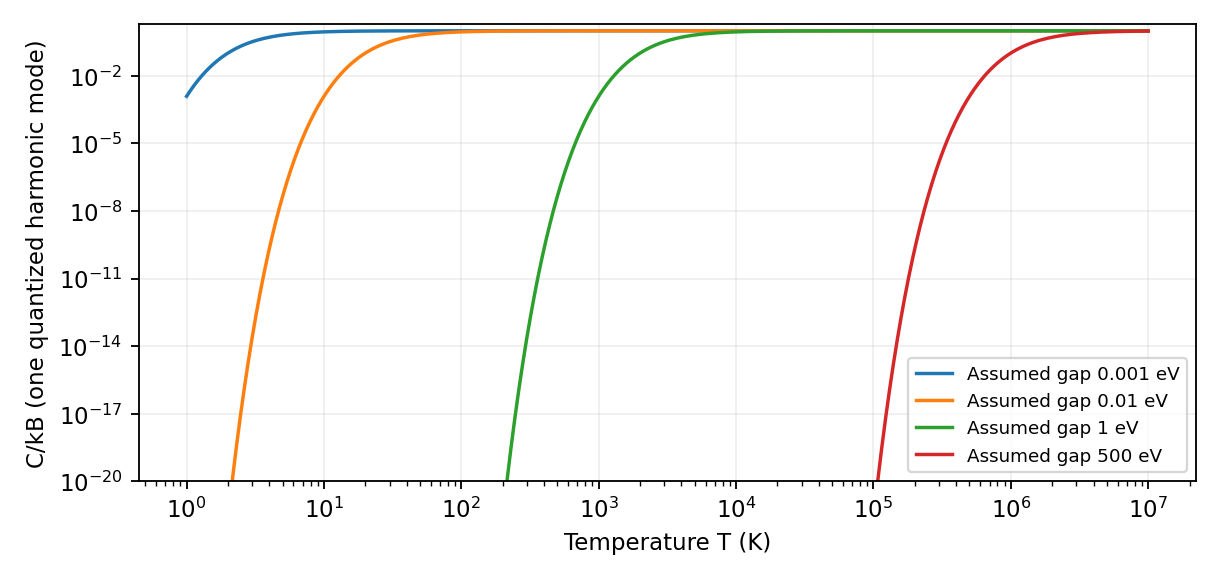
\includegraphics[width=.88\linewidth]{figures/conditional_bose_heat_capacity.png}
\caption{Heat capacity predicted after \emph{assuming} independent quantized oscillator gaps. This does not establish either the existence or value of a Kelvin gap.}
\end{figure}

If there are finitely many independent oscillators $j=1,\dots,N$ with energies $\Delta_j\ge\Delta_*>0$, then monotonicity of $f(\Delta)=\Delta/(e^{\beta\Delta}-1)$ yields the exact conditional bound
\begin{equation}
0\le U_{\rm total}\le N\frac{\Delta_*}{e^{\Delta_*/(k_BT)}-1}.
\end{equation}
The manuscript's $N\Delta_* e^{-\Delta_*/k_BT}$ is a low-temperature asymptotic estimate, not a strict upper bound at finite temperature.

The condition $\Delta_*/(k_BT_{\rm eff})\ge60$ at $T_{\rm eff}=10^5\,\mathrm K$ gives $\Delta_*\ge517.040\,\mathrm{eV}$. The dimensionless threshold 60, effective temperature and claimed spectroscopy bound $a_n\le10^{-62}\,\mathrm{J\,K^{-2}}$ are external modeling premises lacking an independently reconstructed measurement contract in these source PDFs. A $T^2$ correction is also not a universal prediction for an arbitrary finite set of Kelvin oscillators.

\subsection{The Schrodinger variational identity is conditional}
The papers insert the energy functional
\[
\mathcal F[\psi]=\int d^3x\left[\frac{\hbar^2}{2m_e}|\nabla\psi|^2+V(\mathbf x)|\psi|^2\right],\quad \int|\psi|^2d^3x=1.
\]
Its stationary variation yields $-\hbar^2\nabla^2\psi/(2m_e)+V\psi=E\psi$, a correct conditional result. Since the quantum gradient coefficient and potential were inserted, this does not derive quantum mechanics from the Euler flow. The status in the registry is \status{VARIATIONAL\_IDENTITY\_ONLY}.

\section{Two-sector field dynamics: two distinct mathematical baselines}
\subsection{Repair of the dissipative rate model}
The dual-vacuum manuscript (p. 4) adds $\kappa_{se}=4Z_s/Z_{\rm bound}$ to inverse lifetimes. Since both $Z$ values have impedance units (Rayl), $\kappa_{se}$ is dimensionless; adding it to rates in ${\rm s^{-1}}$ is invalid. Define a new transfer rate $g\,[\mathrm{s^{-1}}]$ and an efficiency $0\le\eta\le1$. An explicitly energy-accounted \emph{phenomenological} model is
\begin{equation}
\begin{split}
\dot E_s&=-(d_s+g)E_s,\\
\dot E_e&=\eta gE_s-d_eE_e,\\
\dot E_{\rm loss}&=d_s E_s+(1-\eta)gE_s+d_eE_e.
\end{split}
\end{equation}
Thus $d(E_s+E_e+E_{\rm loss})/dt=0$, and all three energy pools remain nonnegative for nonnegative input data. For $E_s(0)=E_0$, $E_e(0)=0$, $a=d_s+g$ and $b=d_e$,
\begin{equation}
E_e(t)=\eta gE_0\frac{e^{-at}-e^{-bt}}{b-a},\qquad
 t_{\rm peak}=\frac{\ln(b/a)}{b-a}.
\end{equation}
For $a^{-1}=0.1\,\mathrm{ns}$ and $b^{-1}=30\,\mathrm{ns}$, this gives $t_{\rm peak}=0.572286\,\mathrm{ns}$: \textbf{not} a 30-ns delayed peak. A separate memory, propagation or gated-detection mechanism would need explicit construction.

\begin{figure}[ht]
\centering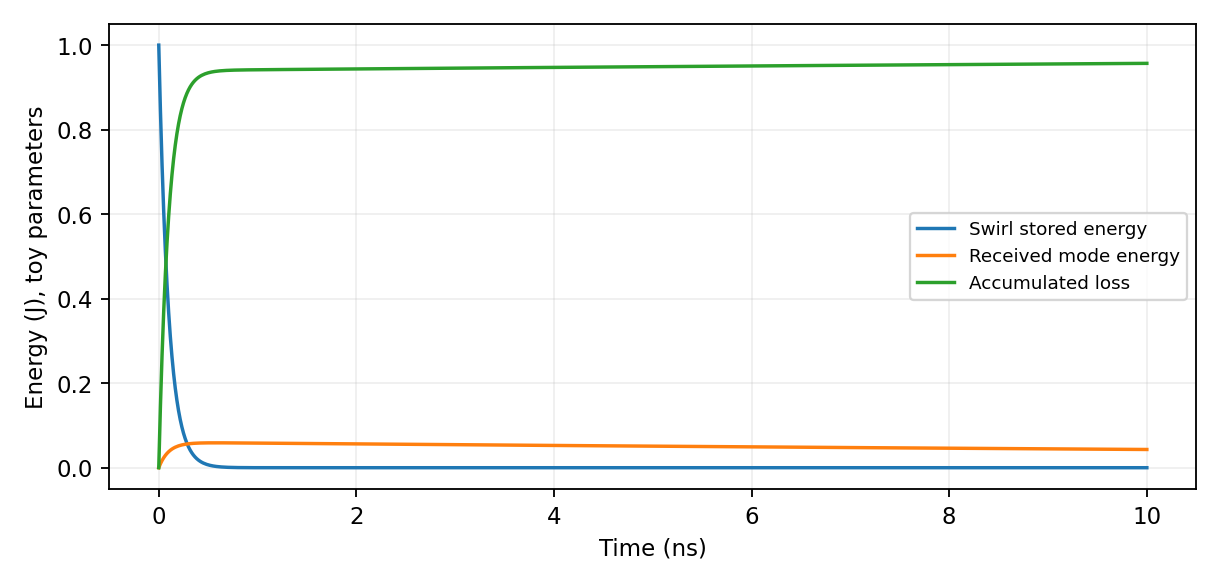
\includegraphics[width=.88\linewidth]{figures/two_sector_energy_balance.png}
\caption{Energy-accounted \emph{irreversible toy} rates with $g=10^9\,\mathrm{s^{-1}}$, $d_s=9\times10^9\,\mathrm{s^{-1}}$, $d_e=(30\,\mathrm{ns})^{-1}$, $\eta=0.6$, $E_0=1\,\mathrm J$. Total accounted energy stays 1 J. No claim that these parameters describe nature.}
\end{figure}

\subsection{Conservative coupled-mode action: independent construction}
An equally useful, fully conservative \emph{mathematical} model uses displacement-like variables $q_s,q_e$ (metres), masses $M_s,M_e$ (kg), stiffnesses $k_s,k_e,g$ (N/m), and Lagrangian
\begin{align}
L=&\frac{M_s}{2}\dot q_s^2+\frac{M_e}{2}\dot q_e^2-\frac{k_s}{2}q_s^2
 -\frac{k_e}{2}q_e^2-\frac{g}{2}(q_s-q_e)^2,\\
H=&\frac{p_s^2}{2M_s}+\frac{p_e^2}{2M_e}+\frac{k_s}{2}q_s^2+
\frac{k_e}{2}q_e^2+\frac{g}{2}(q_s-q_e)^2,\qquad p_i=M_i\dot q_i.
\end{align}
$H\ge0$ when all $M_i,k_i>0$ and $g\ge0$. The squared eigenfrequencies are the two eigenvalues of $M^{-1/2}KM^{-1/2}$ with
\[
M=\begin{pmatrix}M_s&0\\0&M_e\end{pmatrix},\quad
K=\begin{pmatrix}k_s+g&-g\\-g&k_e+g\end{pmatrix}.
\]
The included velocity-Verlet integrator checks conservative energy drift and second-order time convergence. \textbf{No} physical identity between $q_e$ and the electromagnetic vector potential, or between $q_s$ and PKLSA vorticity, is implied by this oscillator baseline. This baseline is separate from the coarse-grained rate equations.

\subsection{Faraday coupling and constitutive closure}
The source expression $-G\partial_t(\nabla\times\vfield)\hat{\mathbf n}$ is not a well-defined vector without specifying a contraction/operator. One may \emph{define} $\mathbf B_{\rm eff}=\mathbf B+\chi\om$ with $[\chi]=\mathrm{T\,s}$. Then $\nabla\cdot\mathbf B_{\rm eff}=0$ follows from $\nabla\cdot(\nabla\times\vfield)=0$. This is only a field redefinition. A genuine electromagnetic theory additionally needs independent dynamical/constitutive equations, gauge symmetry, energy exchange, and testable consequences. Likewise the characteristic ratio $c/v_{\rm swirl}\approx274$ is arithmetic; a tangential swirl speed is not automatically an independent signal speed.

\section{Qualification gates for source-native PKLSA}
\begin{tabular}{@{}p{0.12\linewidth}p{0.51\linewidth}p{0.31\linewidth}@{}}\toprule
Gate & Test & Current state\\\midrule
K0 & Immutable provider, exact 3D seed and core model manifest & NOT CONNECTED\\
K1 & True ring/trefoil equilibrium or relative periodic orbit & NOT RUN\\
K2 & Linearized Kelvin/Floquet spectrum with symmetry modes projected out & NOT RUN\\
K3 & Spatial $N=1200,2400$ and $4800,9600$ plus independent time refinement & NOT RUN\\
K4 & Extra gap versus finite-length mode spacing; source-native circulations & NOT RUN\\
K5 & Optional quantization/thermal bath separately qualified & NOT RUN\\
D0 & Conservative two-mode Hamiltonian numerical tests & MATH PASS\\
D1 & Coarse-grained energy-rate positivity and dimensional tests & MATH PASS\\
D2 & Source-native torsional mode / EM constitutive coupling & UNRESOLVED\\\bottomrule
\end{tabular}

\section{Deliverables and validation meaning}
Original \texttt{v0.1.0} outputs, raw extracted equations, and 11 source files are retained. This addendum contributes 22 claim records and independent numerical outputs (\texttt{kelvin\_periodic\_proxy.csv}\allowbreak, \texttt{conditional\_thermal\_grid.csv}\allowbreak, \texttt{two\_sector\_energy\_rate\_example.csv}\allowbreak, \texttt{conservative\_oscillator\_energy\_trace.csv}). \texttt{run\_all.cmd} rebuilds the entire index and addendum and executes 55 mathematical regressions. None is a native PKLSA or experimental certification.

\section*{References}
\begin{thebibliography}{99}
\bibitem{Saffman1992} P. G. Saffman, \emph{Vortex Dynamics}, Cambridge University Press (1992). DOI: \href{https://doi.org/10.1017/CBO9780511624063}{10.1017/CBO9780511624063}.
\bibitem{Fetter2009} A. L. Fetter, ``Rotating Trapped Bose--Einstein Condensates'', \emph{Rev. Mod. Phys.} \textbf{81}, 647--691 (2009). DOI: \href{https://doi.org/10.1103/RevModPhys.81.647}{10.1103/RevModPhys.81.647}.
\bibitem{Pathria2011} R. K. Pathria and P. D. Beale, \emph{Statistical Mechanics}, 3rd ed., Elsevier (2011). ISBN: 9780123821881.
\bibitem{Kelvin1880} W. Thomson (Lord Kelvin), ``Vibrations of a Columnar Vortex'', \emph{Philosophical Magazine} \textbf{10}, 155--168 (1880). \href{https://archive.org/details/philosophicalmag10lond}{Archive permalink}.
\bibitem{IskandaraniKelvin2025} O. Iskandarani, ``Suppression of Kelvin-Mode Thermodynamics in Atomic Orbitals: A Gapped Vortex-Filament Resolution in Swirl--String Theory'', manuscript (14 December 2025), supplied PDF.
\bibitem{IskandaraniKelvin2026} O. Iskandarani, ``Kelvin Mode Suppression in Atomic Orbitals: A Vortex-Filament Gap'', supplied manuscript, 10 pp. (date not specified in this PDF).
\bibitem{IskandaraniDual2025} O. Iskandarani, ``Hydrodynamic Dual-Vacuum Unification: Swirl Superradiance, Photon Torsion, and the Unruh Echo Mechanism'', manuscript (1 December 2025), supplied PDF.
\end{thebibliography}
\end{document}
